\section{Concave Clique Likelihoods}
\label{sec:piecewise}

The method of moments approach to recover parameters for each clique
  $\sC$ presented in the previous section is easy to understand and
  analyze, but sensitive to noise. 
In this section we propose an alternate solution, optimizing the 
  likelihood for each clique, that is more robust to noise.
We show that under the same conditions as \algorithmref{directed}, the
  clique likelihoods are strictly concave, guaranteeing that
  gradient-based optimization will converge to the unique global
  optimum.

Consider a clique $\sC = \{h_{i_1}, \cdots h_{i_m}\} \in \sG$, with
  exclusive views $\sV = \{x_{v_1}, \cdots, x_{v_m}\}$. 
The piecewise likelihood of $\Sx{\sV}$ is,
\begin{align*}
  \sL_\ml(\Sx{\sV}) 
   &= \sum_{\vx \in \sD} \log \Pr( \Sx \sV ) \\
   &= \sum_{\vx \in \sD} \log \sum_{\Sh \sC} \Pr( \Sx \sV \given \Sh \sC ) \\
   &= \sum_{\vx \in \sD} \log \mH_\sC(\mOpp{v_1}{i_1} [x_{v_1}], \cdots, \mOpp{v_m}{i_m} [x_{v_m}])
\end{align*}

For this section, it will be convenient to represent $\mH_\sC$ as
  a vector in $\Re^{k^m}$, and represent $\mOpp{\sV}{\sC} \eqdef
  \mOpp{v_1}{i_1} [x_{v_1}] \otimes \cdots \otimes
  \mOpp{v_m}{i_m} [x_{v_m}]$ as a matrix in $\Re^{k^m \times
  d^m}$.
Then the likelihood objective is,
\begin{align*}
  \sL_\ml(\Sx{\sV}) 
   &= \sum_{x \in \sD} \log \mOppt{\sV}{\sC}[\vx] \mH_\sC,
\end{align*}

The likelihood is concave in $\mH_\sC$; next, we show that it is
strictly concave, which guarantees that it has a unique maximizer.
  
Taking the first derivative,
\begin{align}
  \grad_{\mH_\sC} \sL_\ml(\sX_\sV) 
  &= \sum_{x \in \sD} \frac{\mOpp{\sV}{\sC}_x}{\mH_\sC \cdot \mOpp{\sV}{\sC}[\vx]} \nonumber \\ 
  &= \mOpp{\sV}{\sC}[\vx] \diag(\tilde \mO_{\sV})^{-1} \mO_{\sV}, \label{eqn:lhood-grad}
\end{align}
where $\tilde \mO_\sV$ is marginal distribution with parameters $\mH_\sC$, also represented as a vector in $\Re^{d^m}$.

Taking the second derivative.
\begin{align}
  \grad^2_{\mH_\sC} \sL_\ml(\Sx \sV) 
  &= \sum_{x \in \sD} \frac{\mOpp{\sV}{\sC}[\vx] \mOppt{\sV}{\sC}[\vx]}{(\mH_\sC \cdot \mOpp{\sV}{\sC}[\vx])^2} \nonumber \\
  &= \sum_{x \in \sD}\mOpp{\sV}{\sC}[\vx] \mOppt{\sV}{\sC}[\vx] \frac{\mO_{\sV}[\vx]}{\tilde \mO_{\sV}^2[\vx]} \nonumber \\
  &= \mOpp{\sV}{\sC} \diag(\mO_{\sV}) \diag(\tilde \mO_{\sV})^{-2} \mOppt{\sV}{\sC}. \label{eqn:lhood-hess}%
\end{align}

It follows that $\grad^2_{\mH_\sC} \sL_\ml(\Sx \sV) \succ 0$ because
$\tilde \mO_\sV, \tilde \mO_\sV \succ 0$ and $\mOpp{\sV}{\sC}$ is
full rank and stochastic.

\algorithmref{piecewise} reviews our algorithm.

\begin{algorithm}
  \caption{\LearnPiecewise}
  \label{algo:piecewise}
  \begin{algorithmic}
    \REQUIRE A graphical model $\sG$ satisfying \propertyref{bottleneck}, data $\sD$
    \ENSURE Marginals $Z_\sC$ for every clique $\sC \in \sG$
\STATE Identify exclusive views $x_\sV = \{x_{v_1}, \cdots, x_{v_m}\}$.
\STATE $\hat \mH_\sC = \arg\max_{\mH_\sC \in \Delta_{k^m-1}} \sum_{\Sx \sV} \log  \mOppit{\sV}{\sC}[\Sx \sV] \mH_\sC$.
%      Run expectation-maximization to convergence on the piecewise likelihood \eqref{eqn:piecewise}, over data $\{\vec x_\sC : x \in \sD\}$
  \end{algorithmic}
\end{algorithm}

\subsection{Comparison with Method of Moments}

The Cramer-Rao bound tells us that this is statistically the most
  efficient estimator we can get for $Z_\sC$. 
We also study the efficiency of the method of moments estimator.

\begin{lemma}(Asymptotic variance for the likelihood)
  \label{lem:pw-variance}
  The asymptotic variance in the recovered parameters $Z_{\sC}$ by optimizing the likelihood is,
  \begin{align*}
    \Sigma^{(\ml)} &= \mOppit{\sV}{\sC} \diag(M_\sV) \Sigma_\sV \diag(M_\sV) \mOppi{\sV}{\sC},
  \end{align*}
  where $\Sigma_\sV$ is the variance of the moment estimates, 
  \begin{align*}
    \Sigma_\sV &= \diag(M_\sV) - M_\sV M_\sV^\top.
  \end{align*}
\end{lemma}
\begin{proof}
  Using the delta-method \cite{vaart98asymptotic}, we have that the
  asymptotic distribution of $Z_\sC$ is,
  \begin{align*}
    \sqrt{n}(\hat Z_{\sC} - Z_{\sC}) &\convind \sN( 0, \\
      &\quad \grad^2 \sL_\ml(\vec x_\sC)^{-1} \Var[\grad \sL_\ml(\vec x_\sC)] \grad^2 \sL_\ml(\vec x_\sC)^{-1}).
  \end{align*}

  From \equationref{lhood-grad}, we get
  \begin{align*}
    \Var [\grad \sL_\ml(\vec x_\sC)] &= \mOpp{\sV}{\sC} \diag(\tilde M_\sV) \Sigma_\sV \diag(\tilde M_\sV) \mOpp{\sV}{\sC}^T .
  \end{align*}

  Finally, using \equationref{lhood-hess}, we have
  \begin{align*}
    \Sigma_{Z_\sC} 
      &= \grad^2 \sL_\ml(\vec x_\sC)^{-1} \Var [\grad \sL_\ml(\vec x_\sC)] \grad^2 \sL_\ml(\vec x_\sC)^{-1}) \\
      &= \pinvt{\mOpp{\sV}{\sC}} \diag(\tilde M_\sV) \Sigma_\sV \diag(\tilde M_\sV) \pinv{\mOpp{\sV}{\sC}}.
  \end{align*}

  At the true parameters, $\tilde M_\sV = M_\sV$, completing the proof.
\end{proof}

\begin{corollary}
  The asymptotic variance of optimizing the log-likelihood, $\Sigma_p$
  is strictly less than that of the moment-matching objective
  $\Sigma_m$; $\Sigma_p \succ \Sigma_m \succ 0$.
\end{corollary}
\begin{proof}
  From \lemmaref{mom-variance}, we have the asymptotic variance of the method of moments estimator, $\hat Z_\sC^{(\mom)}$ is,
  \begin{align*}
    \Sigma^{(\mom)} &= \mOppit{\sV}{\sC} \Sigma_\sV \mOppi{\sV}{\sC},
  \end{align*}

  By \lemmaref{pw-variance}, we have the asymptotic variance of the piecewise likelihood estimator, $\hat Z_\sC^{(\ml)}$ is,
  \begin{align*}
    \Sigma^{(\ml)} &= \mOppit{\sV}{\sC} \diag(M_\sV) \Sigma_\sV \diag(M_\sV) \mOppi{\sV}{\sC},
  \end{align*}

  Note that $\Tr(\diag M_\sV) = 1$ as it represents the marginal
  distribution of $\sV$; thus, $\Sigma^{(\mom)} \succ \Sigma^{(\ml)}
  \succ 0$.  Finally the asymptotic efficiency of the method of moments
  estimator is, 
  \begin{align*}
    e^\mom &= \Tr( \Sigma^{(\ml)}\Sigma^{(\mom) -1} )  \\
           &= \Tr( \diag(M_\sV) \Sigma_\sV \diag(M_\sV) \Sigma_\sV^{-1} ).
  \end{align*}
\end{proof}

\paragraph{Intuition}
It is well known that the method of moments estimator is less
  statistically efficient than the maximum likelihood estimator. 
To get a sense for how large the gap is, consider an example where in
  $M_\sV$ is close to the uniform distribution, i.e. $\diag(M_\sV)
  = \frac{1}{d} I$. 
Then the efficiency of the $e^\mom = \Tr(\frac{1}{d^2} I)
  = \frac{1}{d}$.
In other words, the gap in variance between the method of moments
  estimator and maximum likelihood grows as an order of $d$.

For another view of this phenomenon, consider the objective function
  associated with the method of moments, 
\begin{align*}
  \sL_\mom(\Sx \sV) &= \half \|Z_\sC \mOpp{\sV}{\sC} - M_\sV \|_F^2.
\end{align*}
In comparison, the negative log-likelihood objective is much more
concave, so we expect it to be more efficient. 
\figureref{piecewise-objective} compares the objective values for
different choices of the $\pi$ parameter in a hidden Markov model
\figureref{examples-hmm} with 2 states ($k=2$) and $d=10$ dimensions.

\begin{figure}
  \centering
  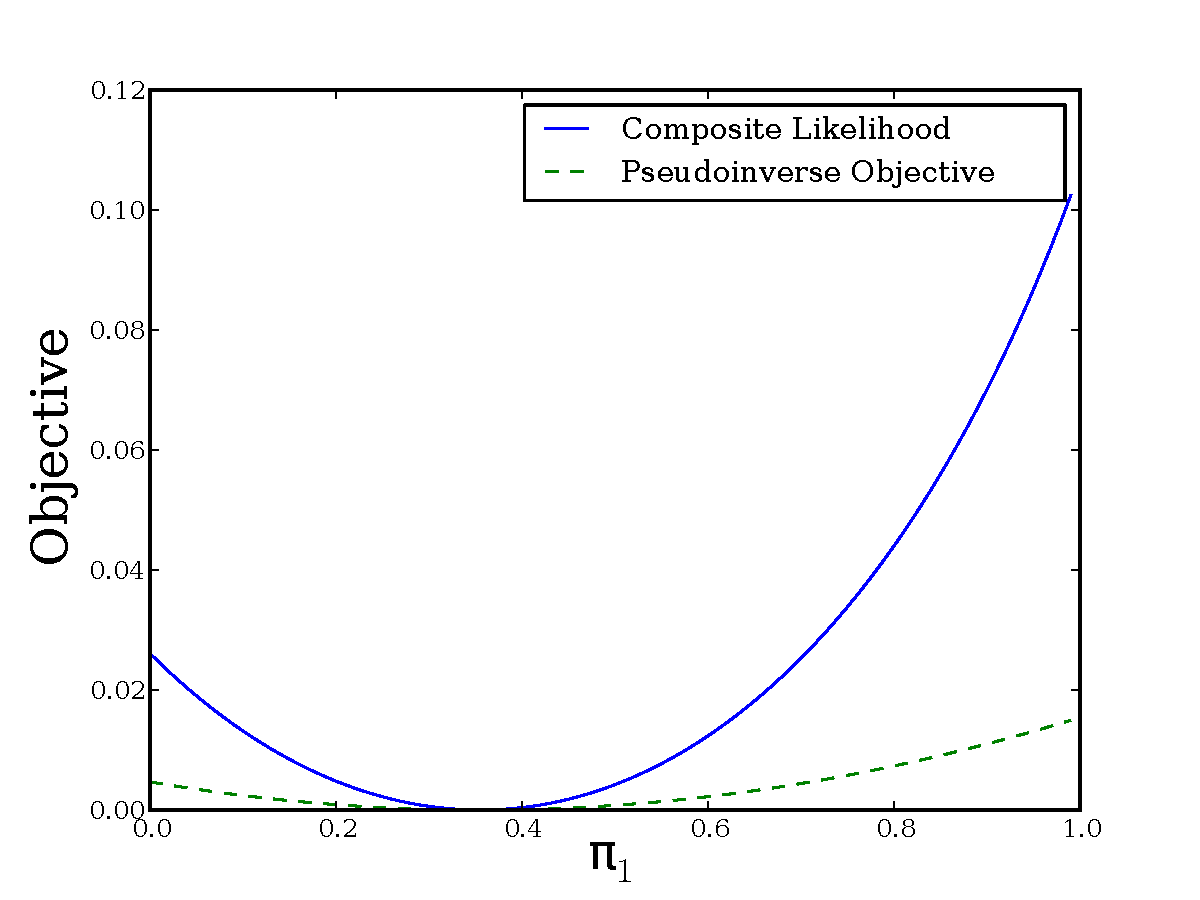
\includegraphics[width=\columnwidth]{figures/piecewise-objective.pdf}
  \caption{Comparing the piecewise objective with the moment-matching objective for just one parameter}
  \label{fig:piecewise-objective}
\end{figure}

\subsection{More examples}

We will now instantiate our algorithm for a couple more examples, illustrated in \figureref{examples}.

\begin{figure}
  \subfigure[Hidden Markov Model] {
    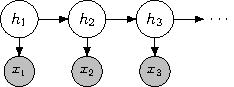
\includegraphics{figures/hmm.pdf}
    \label{fig:examples-hmm}
  }
%  \subfigure[Directed grid model] {
%    \label{fig:examples-grid}
%    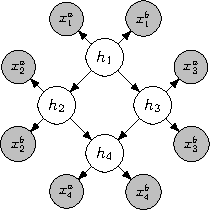
\includegraphics{figures/grid.pdf}
%  }
  \subfigure[Tree model] {
    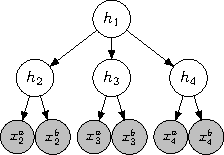
\includegraphics{figures/tree.pdf}
    \label{fig:examples-tree}
  }
  \caption{Additional examples of models learnable using \LearnMarginals \todo{Label parameters}}
  \label{fig:examples}
\end{figure}

\paragraph{Hidden Markov Model}

In this example (\figureref{examples-hmm}), we assume that
  $\Pr(x_i|h_i) = O  ~\forall i$  and that $\Pr(h_{i+1} | h_i)
  = T ~\forall i$ (i.e. we have parameter sharing).
Note that while the first (and last) hidden variables $h_1, h_T$ in the
  sequence are not bottlenecks, they still have exclusive views ($x_1$ and
  $x_T$ respectively) whose parameters we know because they share
  parameters, $O$.
In step 1 of our algorithm, we use the bottleneck $h_2$ with views $x_1,
  x_2, x_3$ and solve $O$.
In step 2 of our algorithm, we can recover $\pi$ by solving for the
  unary clique $\{h_1\}$ and recover $T$ from the clique $\{h_{1},
  h_{2}\}$.

\paragraph{Latent Tree Structure}

In the latent tree structure (\figureref{examples-tree}), let the
  parameters be $\Pr(h_i) = \pi$, $\Pr(h_i | h_1) = T ~i \in \{2,3,4\}$
  and $\Pr(x^a_i | h_i) = \Pr(x^b_i | h_i) = O ~i \in \{2,3,4\}$.
Note that while $h_1$ is not directly connected to an observed variable,
  it is still a bottleneck, with views $x^a_2, x^a_3, x^a_4$.

In step 1, we recover the parameters $O$ from the bottleneck $h_2$ with
  views $\{x^a_2, x^b_2, x^a_3\}$. We also recover the conditional moments
  $\mOpp{2}{1}$, $\mOpp{3}{1}$, $\mOpp{4}{1}$ for $h_1$. 
In step 2, we can recover $\pi$ from the clique $\{h_1\}$, using any
  one of views (they are all exclusive). 
To recover $T$ from the clique $\{h_1, h_2\}$, we use the views $x^a_2$
  (exclusive to $h_2$) and $x^a_3$ (exclusive to $h_3$). Note that while
  $x^a_3$ is also a view for $h_2$, $x^a_3$ is independent of $h_2$ given
  $h_1$.

\paragraph{Aggregating observations}
We describe two practical considerations to use samples more efficiently.
Firstly, if we have multiple exclusive views for a hidden variable,
  intuitively, it is better to aggregate over them. 
For example, consider a hidden variable $h_1$ with multiple exclusive
  views $x_1$ and $x_2$.
With the method of moments perspective, to learn the marginal
  distribution over $h_1$, one must solve the following reconstruction
  problem, 
\begin{align*}
  \hat Z_{h_1} &= \arg\min_{Z_{h_1}} \half \|Z_{h_1} \mOpp{1}{1} - M_1 \|^2 + \half \|Z_{h_1} \mOpp{2}{1} - M_2 \|^2,
\end{align*}
which does not have a closed form solution. 
In contrast, this naturally fits into the convex optimization framework, where $\hat Z_{h_1}$ will now be,
\begin{align*}
  \hat Z_{h_1} &= \arg\min_{Z_{h_1}} \sum_{\vx \in \sD} \log Z_{h_1}( \mOpp{1}{1}[x_1] \cdot \mOpp{1}{1}[x_1] ),
\end{align*}
where $\cdot$ denotes element-wise multiplication.
An important note to make is that \TensorFactorize only returns
  a solution up to permutation; if $\mOpp{1}{1}$ and
  $\mOpp{1}{2}$ do not belong to the same bottleneck (e.g. $x^a_2$ and
  $x^b_2$ in \figureref{examples-tree}), then some
  care must be taken to ensure they have the same labelling.

Secondly, we can exploit parameter sharing by aggregating over
  disjoint sets of observed variables. 
For example, in \figureref{examples-hmm}, we can aggregate the statistics for
  bottlenecks $h_i$ with views $\{x_{i-1}, x_{i}, x_{i+1}\}$ before
  running \TensorFactorize; this will give us a consistent estimate for
  $O$ (as well as $T$).

